\documentclass[openany,oneside]{book}
\usepackage[utf8]{inputenc}
\usepackage[italian]{babel}

% url
\usepackage{url}

% minted
\usepackage{minted, subcaption, cancel, afterpage,multicol}
\newminted{javascript}{escapeinside=||,mathescape=true,linenos}

% appendix
\usepackage[toc]{appendix}
\renewcommand{\appendixtocname}{Appendici}

% font
\usepackage{microtype}
\usepackage{textcomp}
\usepackage{stmaryrd}

% figure
\usepackage{subcaption}

% math-generic
\usepackage{mathtools,amsmath,amssymb,amsfonts,galois}

% math-theorems
\usepackage{amsthm}
\newtheorem{theorem}{Teorema}
\theoremstyle{definition}
\newtheorem{definition}[theorem]{Definizione}
\newtheorem{example}[theorem]{Esempio}

% BIBLIOGRAPHY ====================
\usepackage[backend=biber,style=numeric,sorting=ynt]{biblatex}
\addbibresource{biblio.bib}

% commands
\usepackage{xparse}
\newcommand{\N}{\mathbb{N}}
\newcommand{\Z}{\mathbb{Z}}
\newcommand{\semantics}[1]{\llbracket #1 \rrbracket}
\newcommand{\set}[1]{\mathrm{#1}}
\newcommand{\term}[1]{\mathrm{#1}}
\newcommand{\fun}[1]{\mathit{#1}}
\newcommand{\struct}[1]{\langle #1 \rangle}

\NewDocumentCommand{\NewCustomOperator}{o o m m m}{
    \IfNoValueTF{#1}{
        #3
    }{
        \IfNoValueTF{#2}{
            #4 #1
        }{
            #1 #5 #2
        }
    }
}

\NewDocumentCommand{\meet}{o o}{
    \NewCustomOperator[#1][#2]{\sqcap}{\bigsqcap}{\sqcap}
}

\NewDocumentCommand{\join}{o o}{
    \NewCustomOperator[#1][#2]{\sqcup}{\bigsqcup}{\sqcup}
}

\title{Implementazione di tool per l'interpretazione astratta di codice Javascript }
\author{Massimiliano Incudini}
\date{Maggio 2018}

\begin{document}

\maketitle

\setcounter{tocdepth}{1}
\tableofcontents

\chapter{Analisi statica}

Per verificare la correttezza dei programmi e la loro conformità alle specifiche vengono utilizzate diverse tecniche. Le due principali sono l'\emph{analisi dinamica} e l'\emph{analisi statica}. La prima consiste nell'eseguire il programma per qualche input fissato ed osservarne i risultati. La seconda consiste nel processare il codice sorgente del programma senza eseguirlo, e l'output del processo saranno le proprietà che valgono per il tale sorgente. Quest'ultima ha il vantaggio che le proprietà ricavate valgono per ogni input. 

\begin{definition}[Programma]
Un \emph{programma} è una sequenza finita di istruzioni codificate all'interno di un certo formalismo.
\end{definition}

Per noi l'esecuzione di un programma equivale all'esecuzione di una \emph{macchina di Turing} (MdT) che implementa tale programma. L'insieme di tutte le MdT $\{ M_i \}_{i \in \N}$ è numerabile, ed ad ognuna di esse è assegnato un indice. Ogni MdT è equivalente all'esecuzione di una funzione parziale ricorsiva $\phi_i$. Per le definizioni formali di MdT e funzione parziale ricorsiva vedere \cite{calcolability}.

\begin{definition}[Proprietà]
Una proprietà $\Pi$ sulle MdT è un sottoinsieme di $\{ M_i \}_{i \in \N}$. Poichè ad ogni MdT è associato un indice, possiamo equivalentemente definire $\Pi$ sottoinsieme di $\N$.
\end{definition}

Alcuni esempi di proprietà sono $\Pi_1 = \{ i \mid M_i \text{ non effettua divisioni per zero} \}$ oppure $\Pi_2 = \{ i \mid \text{il programma di } M_i \text{ contiene un \texttt{while}} \}$.

\section{Limiti dell'analisi statica}

\begin{definition}[Decidibilità]
Un insieme (o proprietà) $\Pi$ è detto \emph{decidibile} o \emph{ricorsivo} se esiste una MdT $M_\Pi$ tale che per ogni input $p$ restituisca $1$ se $p \in \Pi$ e $0$ se $p \not\in\Pi$. 
\end{definition}

Le proprietà sono estensionali se riguardano in qualche modo il comportamento del programma, quindi le proprietà semantiche. Un esempio è: $\Pi = \{ M_i \mid M_i \text{ termina sempre} \}$. Le proprietà intensionali riguardano invece ``com'è fatto" il programma. Un esempio è $\Pi = \{ M_i \mid \text{il programma di } M_i \text{ contiene un } \texttt{while} \}$.

\begin{definition}[Proprietà estensionale]
Sia $\Pi$ una proprietà sulle MdT. $\Pi$ si dice estensionale se per ogni $x,y\in\N$ si ha
\[ \left( x \in \Pi \; \land \; \varphi_x = \varphi_y \right) \to y \in \Pi \]
dove $\varphi_x = \varphi_y$ è la notazione che abbrevia $\forall z . \varphi_x(z)= \varphi_y(z)$.
\end{definition}

Un importante teorema dice che la maggior parte proprietà semantiche (estensionali) che vorremmo provare non sono decidibili.

\begin{theorem}[Teorema di Rice]
Ogni proprietà estensionale è decidibile se e solo se è banale (uguale all'insieme vuoto oppure a tutto $\N$).
\end{theorem}

Nonostante questo risultato negativo, esistono molte tecniche per estrarre proprietà semantiche \emph{approssimate}.

\section{Soundness e completeness}

\begin{definition}[Soundness]
L'analizzatore è detto \emph{consistente} o \emph{sound} se approssima per eccesso il comportamento del programma.
\end{definition}
In questo caso, dati in input $\Pi$ ed $M$, riporto tutte le violazioni della proprietà $\Pi$ ma alcune di queste potrebbero essere falsi allarmi.

\begin{definition}[Completeness]
L'analizzatore è detto \emph{completo} o \emph{complete} se approssima per difetto il comportamento del programma.
\end{definition}
In questo caso, dati in input $\Pi$ ed $M$, tutte le violazioni della proprietà $\Pi$ che riporto sono ``vere violazioni", non è detto però che queste siano tutte (posso avere falsi negativi). La situazione ideale sarebbe avere un analizzatore sia \emph{sound} che \emph{complete}. Questo molte volte non è possibile: per il teorema di Rice, le proprietà decidibili sono solo quelle banali, da qualche parte devo effettuare approssimazioni.


\chapter{Interpretazione astratta}

L'interpretazione astratta è una tecnica di analisi statica che consiste nel definire un approssimazione \emph{corretta} e \emph{decidibile} della semantica del programma da analizzare. Compare per la prima volta nel paper \cite{cousot} di P.~Cousot e R.~Cousot del 1977. 

\section{Semantica}

\begin{definition}[Semantica]
La semantica di un programma $P$ è la descrizione formale di come il programma viene eseguito attraverso una macchina. Si denota con $\semantics{P}$. 
\end{definition}

I programmi scritti in linguaggi imperativi sono composti da istruzioni che vengono eseguite in sequenza. Ad ogni step di computazione, la macchina aggiorna una tabella detta \emph{memoria} di associazioni variabile\textrightarrow{}valore. 

La semantica che descrive i programmi dovrà formalizzare il concetto di \emph{esecuzione di una istruzione}. Una rappresentazione efficace è quella del \emph{control flow graph}.

\begin{definition}[Control flow graph]
Il control flow graph è un grafo $\struct{V, E \subseteq V \times V}$ tale che l'insieme $V = \set{Point}$ dei vertici sono i punti del programma e l'insieme $E$ degli archi è l'insieme delle istruzioni. 
\end{definition}

\begin{definition}[Sistema di transizioni]
Un \emph{sistema di transizioni} è una struttura $\struct{\mathbf{S}, \to}$ del programma $P$ dove $\mathbf{S}$ è un insieme di stati (``fotografie" della memoria in un certo istante) ed $\to$ è una relazione binaria tra stati tale che
\[ \sigma \to \sigma' \iff \sigma' \text{ è un possibile successore di } \sigma; \quad \sigma, \sigma' \in \mathbf{S} \]
\end{definition}
La relazione $\to$ formalizza il concetto di step di esecuzione. Una sequenza di stati $\sigma_0 \sigma_1 ... \sigma_n$ è detta \emph{trace}. Ogni trace rappresenta una esecuzione di un programma è può anche essere infinita. Da questa si può definire la \emph{trace semantics} (per approfondimenti vedi \cite{xavier}).

\subsection{Trace semantics}

\begin{definition}[Trace semantics]
Dato un sistema di transizioni $\struct{\mathbf{S}, \to}$ del programma $P$ è definita la trace semantics $\semantics{\mathbf{S}}$ come l'insieme delle possibili tracce di esecuzione di $P$:
\[ \semantics{\mathbf{S}} = \{ \sigma_0 \sigma_1 ... \sigma_n \mid \forall i \;\, \sigma_i \in \mathbf{S} \land (\sigma_i \to \sigma_{i+1}) \} \]
\end{definition}

Guardando la trace semantics possiamo vedere in ogni momento dell'esecuzione di un programma se una certa proprietà vale o no. Noi preferiremmo non essere legati alle informazioni temporali che porta con se la trace. Definiamo quindi una semantica che evidenzia le \emph{invarianti} presenti in ogni punto dell'esecuzione. 

\subsection{Collecting semantics}

\begin{definition}[Collecting semantics]
La collecting semantics di un programma $P$ rappresentato dal control flow graph $\struct{\set{Point}, E}$ è una funzione
\[ \mathcal{CS} : \set{Point} \to \wp(\set{State}) \]
che associa ad un punto del programma l'insieme dei possibili stati che può avere.
\end{definition}

Conoscendo la collecting semantics di $P$ possiamo facilmente verificare se la nostra proprietà vale o meno. $\mathcal{CS}$ può essere ricavata tramite un algoritmo di fixpoint iterativo (per approfondire vedi Sezione~\ref{sec:fixpoint}). 

\begin{example}\label{example:collecting}
Calcola la collecting semantics del seguente pezzo di codice.
\begin{javascriptcode}
x = 0;
y = 2;
while (x < 3) {
    y = y * y;
    x = x + 1;
}
\end{javascriptcode}
Lo stato che dobbiamo mantenere è una coppia $\struct{x,y}$ che all'inizio ha valore $\set{INIT} = \{ \struct{0, 2} \}$. La funzione di cui dobbiamo trovare il least fixed point è
\[ P(M) = \texttt{WHILE}_{x<3}(\texttt{INCX}(\texttt{SQUAREY}(M)), \set{INIT}) \]
con 
\begin{align*}
    \texttt{SQUAREY}(M) &= \{ \struct{x,y^2} \mid \struct{x,y} \in M \} \\
    \texttt{INCX}(M) &= \{ \struct{x+1,y} \mid \struct{x,y} \in M \} \\
    \texttt{WHILE}_{x<3}(M, I) &= (M \cup I) \cap \{ \struct{x,y} \mid x < 3 \} 
\end{align*}

Procediamo col metodo iterativo:
\begin{align*}
    P(\varnothing) 
        &= (\texttt{INCX}(\texttt{SQUAREY}(\varnothing)) 
        \cup \{ \struct{0, 2} \} ) 
        \cap \{ \struct{x,y} \mid x < 3 \} \\
        &= \{ \struct{0, 2} \} \\
    P(\{ \struct{0, 2} \}) 
        &= (\texttt{INCX}(\texttt{SQUAREY}(\{ \struct{0, 2} \})) 
        \cup \{ \struct{0, 2} \} ) 
        \cap \{ \struct{x,y} \mid x < 3 \} \\
        &= \{ \struct{0, 2},  \struct{1, 4} \} \\
    P(\{ \struct{0, 2},  \struct{1, 4} \}) 
        &= (\texttt{INCX}(\texttt{SQUAREY}(\{ \struct{0, 2},  \struct{1, 4} \})) 
        \cup \{ \struct{0, 2} \} ) 
        \cap \{ \struct{x,y} \mid x < 3 \} \\
        &= \{ \struct{0, 2},  \struct{1, 4}, \struct{2, 16} \} \\
    P(\{ \struct{0, 2},  \struct{1, 4}, \struct{2, 16} \} ) 
        &= (\texttt{INCX}(\texttt{SQUAREY}(\struct{0, 2},  \struct{1, 4}, \struct{2, 16})) 
        \cup \{ \struct{0, 2} \} ) 
        \cap \{ \struct{x,y} \mid x < 3 \} \\
        &= \{ \struct{0, 2},  \struct{1, 4}, \struct{2, 16}, \struct{3, 64} \}
        \cap \{ \struct{x,y} \mid x < 3 \} \\
        &= \{ \struct{0, 2},  \struct{1, 4}, \struct{2, 16} \}
\end{align*}

Il least fixed point è il valore di memoria $M = \{ \struct{0, 2},  \struct{1, 4}, \struct{2, 16} \}$.
\end{example}

La semantica collecting è però spesso indecidibile. Occorre trovare un modo per renderla decidibile. 

\section{Dominio astratto}

Nell'Esempio~\ref{example:collecting}, la computazione del least fiexed point può diventare molto costosa: gli elementi dell'insieme $M$ sono coppie di tipo $\Z \times \Z$ e il loro numero può velocemente esplodere. Cerchiamo un modo per approssimare $M$. 

\begin{definition}[Dominio]
Il \emph{dominio} è l'insieme dei valori che le variabili possono assumere all'interno dello store. 
\end{definition}

Al posto che mantenere di ogni valore il numero esatto $n \in \Z$, ne manteniamo solamente la parte di informazione che ci interessa.

\begin{example}\label{example:sign}
Il dominio dei segni è definito come segue:
\[ \set{Sign} = \{ \top, \oplus, \ominus, 0, \bot \} \]
dove $\top$ rappresenta un qualsiasi numero, $\oplus$ i numeri positivi o o nulli, $\ominus$ quelli negativi o nulli, $0$ il sono numero zero e $\bot$ nessun numero (usato come condizione d'errore, per esempio la divisione per zero). 
\end{example}

\begin{example}\label{example:interval}
Il dominio degli intervalli è definito come segue:
\[ \set{Interval} = \{ [l,h] \mid l,h \in \Z; \; l \le h \} \]
\end{example}

Entrambi i domini in Esempio~\ref{example:sign} e Esempio~\ref{example:interval} sono approssimazioni del dominio $\wp(\Z)$. I primi due prendono il nome di \emph{dominio astratto} mentre quest'ultimo è detto \emph{dominio concreto}. I domini devono formare una struttura di reticolo completo (per approfondire vedi Sezione~\ref{sec:reticoli}).

\subsection{Connessioni di Galois}\label{sec:galois-c}

Dobbiamo trovare un metodo per passare trasformare gli elementi del dominio concreto in elementi del dominio astratto e viceversa. 

\begin{definition}[Connessione di Galois]
Dati due poset $\struct{C, \le}$ e $\struct{A, \preceq}$, la coppia di funzioni $\struct{\alpha, \gamma}$ viene definita \emph{connessione di Galois} e si indica con 
\[ C \galois{\alpha}{\gamma} A \]
dove
\begin{itemize}
    \item[$C$:] insieme detto dominio concreto;
    \item[$\gamma$:] funzione monotona di concretizzazione $\gamma : A \to C$, $\forall c \in C : c \le \gamma(\alpha(c))$;
    \item[$A$:] insieme detto dominio astratto;
    \item[$\alpha$:] funzione monotona di astrazione $\alpha : C \to A$, $\forall a \in A : a \preceq \alpha(\gamma(a))$.
\end{itemize}
\end{definition}

\begin{example}
Per il dominio di Esempio~\ref{example:sign}, le funzioni $\alpha$ e $\gamma$ sono definite come segue:
\begin{align*}
    \alpha(\varnothing)                                   & = \bot                 &
    \gamma(\bot)                                          & = \varnothing          \\
    \alpha(\{0\})                                         & = 0                    &
    \gamma(0)                                             & = \{ 0 \}              \\
    \alpha(\{ x \mid \min x \ge 0 \}) & = \oplus          &
    \gamma(\oplus)                                        & = \{ x \mid x \ge 0 \} \\
    \alpha(\{ x \mid \max x \le 0 \}) & = \ominus         &
    \gamma(\ominus)                                       & = \{ x \mid x \le 0 \} \\
    \alpha(\{ x \mid \min x < 0 \land \max x > 0\})       & = \top                 &
    \gamma(\top)                                          & = \mathbb{Z}
\end{align*}
\end{example}

\begin{figure}[htbp]
    \centering
    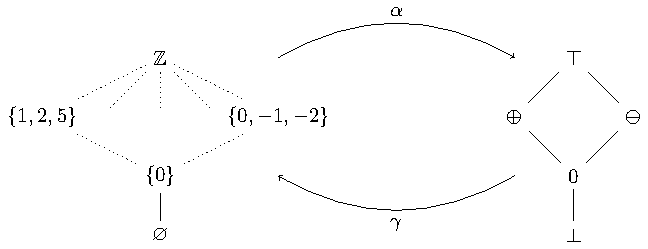
\includegraphics{capitoli/interpretazione-astratta/immagini/reticolo-segni.pdf}
    \caption{Connessione di Galois}
    \label{fig:galois-Z-sign}
\end{figure}

\subsection{Operazioni astratte}

Una volta definito il dominio astratto e la connessione di Galois, per ogni operazione $f : C \to C$ nel dominio concreto dobbiamo definire l'operazione $f^{\#} : A \to A$ nel dominio astratto. Il modo più immediato di definire $f^{\#}$ è tramite la \emph{best correct approximation}.

\begin{definition}[Best correct approximation]
Data una funzione $f : C \to C$ e una connessione di Galois $C \galois{\gamma}{\alpha} A$, si definisce $f^{\#} = \alpha \circ f \circ \gamma$ la \emph{best correct approximation} di $f$ in $A$.
\end{definition}

Tuttavia vorremmo poter avere il risultato di $f^{\#}$ senza dover eseguire $f$. Possiamo definire in un altro modo $f^{\#}$ e poi dimostrarne la correttezza.

\begin{definition}[Correttezza di una funzione astratta]
Data la connessione di Galois $C \galois{\gamma}{\alpha} A$ tra i due poset $\struct{C, \le}$ e $\struct{A, \preceq}$ ed una funzione concreta $f$, la funzione astratta $f^{\#}$ è un'approssimazione corretta di $f$ se vale
\[ \alpha \circ f = f^{\#} \circ \alpha \]
o equivalentemente
\[ f \circ \gamma = \gamma \circ f^{\#} \]
\end{definition}

\begin{example}
Consideriamo la funzione concreta $\fun{add} : \wp(\Z) \times \wp(\Z) \to \wp(Z)$:
\[ \fun{add}(X, Y) = \{ x + y \mid \forall x \in X, \, y \in Y \} \]
Per definire la sua funzione astratta nel dominio dei segni abbiamo più possibilità:
\begin{align*}
    \fun{add}^{\#}_1(s, t) 
    & = \alpha\big(\fun{add}(\gamma(s), \gamma(t)) \big) \\[1em]
    \fun{add}^{\#}_2(s,t) 
    & = \begin{array}{r|ccccc}
        s \downarrow; t \rightarrow & \top & \oplus & \ominus & 0       & \bot  \\\hline
        \top                      & \top   & \top   & \top    & \top    & \bot  \\
        \oplus                    & \top   & \oplus & \top    & \oplus  & \bot  \\
        \ominus                   & \top   & \top   & \ominus & \ominus & \bot  \\
        0                         & \top   & \oplus & \ominus & 0       & \bot  \\
        \bot                      & \bot   & \bot   & \bot    & \bot    & \bot  \\
    \end{array} \\[1em]
    \fun{add}^{\#}_3(s,t) 
    & = \top
\end{align*}
Tutte e tre le varianti sono corrette. 
\end{example}










\chapter{Linguaggio Javascript}

Il linguaggio di programmazione e di scripting Javascript è un linguaggio \emph{multiparadigma} (ad oggetti, imperativo e funzionale), \emph{dinamico} ed \emph{interpretato}. Nasce nel 1995 per la creazione di software web lato client e ad oggi è il più diffuso linguaggio di programmazione al mondo\footnote{\url{http://www.businessinsider.com/the-9-most-popular-programming-languages-according-to-the-facebook-for-programmers-2017-10?IR=T#1-javascript-15}}. 

Il suo essere interpretato, la tipizzazione debole e i casting impliciti portano a produrre software pieno di errori anche difficilmente localizzabili. Queste ragioni motivano l'esistenza del tool. 

\section{Tipi di dato}

I tipi base sono: \emph{numeri}, \emph{booleani} e \emph{stringhe}. I numeri sono tutti valori a 64-bit in virgola mobile. Le stringhe sono sequenze di caratteri Unicode racchiusi tra le doppie virgolette o le virgolette singole ed ammettono alcune sequenze di escape. I caratteri sono stringhe di lunghezza 1. I valori booleani sono \texttt{true} e \texttt{false}. 

I tipi di dato composti sono: \emph{oggetti} e \emph{matrici}. Gli oggetti sono formati da un insieme di proprietà alle quali si accede tramite \texttt{oggetto.proprieta} oppure \texttt{oggetto["proprieta"]}. Le proprietà possono essere aggiunte anche dinamicamente. Gli oggetti sono creati dai costruttori.

Esiste un tipo di dato \emph{Null} il cui unico valore è \texttt{null}. 

Esiste un valore \emph{undefined}. Il test \texttt{x == undefined} è vero se \texttt{x} è stata dichiarata senza mai assegnarne un valore. Il test \texttt{x.prop == undefined} è vero se \texttt{x} è un oggetto che non ha definito la proprietà \texttt{prop}.

\section{Istruzioni}

\section{Costruttori}

\section{Prototype}




\chapter{Realizzazione del tool}

Il codice sorgente Javascript in input viene processato attraverso diverse fasi, in sequenza: parsing, creazione del control flow graph o cfg, analisi, presentazione dei risultati.

\section{Parsing}

Il parsing viene fatto per mezzo della libreria open source Mozilla Rhino. Il risultato del parsing di Rhino è un albero sintattico concreto. Questo viene convertito nell'albero sintattico astratto definito nel package \texttt{it.univr.jsanalyzer.ast}, e i cui componenti sono presenti in \texttt{it.univr.jsanalyzer.builder}.

Tutti gli alberi sintattici e tutti i grafi definiti all'interno del progetto si appoggiano sulle classi della libreria open source GraphStream. Il suo utilizzo ci permette di non \emph{reinventare la ruota}. Inoltre la libreria offre diversi metodi per la visualizzazione dei grafi. 

\section{Componenti dell'albero sintattico astratto}

Ogni nodo dell'albero astratto è uno \texttt{Statement}. Questo rappresenta un'istruzione generica, una linea di codice. La struttura di questo componente è una classe astratta, che viene ereditata e completata dalle classi concrete che rappresentano le istruzioni specifiche (dichiarazione, assegnamento, selezione, ...). 

Le guardie booleane e i valori a destra dell'assegnazione sono \texttt{Expression}. Queste sono definite ricorsivamente attraverso le classi \texttt{UnaryExpression}, \texttt{Binary\-Expression} e \texttt{*Literal}. In casi eccezionali, un'istruzione può essere sia uno Statement che un'Expression, per esempio un'assegnamento che compare all'interno di un'espressione: \mintinline{javascript}{var result = 3 * (a = b)}.

Ad ogni Statement è assegnato un identificatore univoco all'interno dell'albero sintattico. Questo è chiamato \texttt{AbstractPoint} ed è una coppia di interi: \emph{linea di codice} ed \emph{offset}. L'offset è non-zero solo quando lo Statement compare all'interno dell'espressione. All'interno delle espressioni tutti gli Statement vengono enumerati e ad ognuno viene assegnato l'AbstractPoint con la stessa linea ma offset che viene di volta in volta incrementato. Trovi un esempio in Figura~\ref{fig:realizzazione:label-hierarchy}.

\begin{figure}[htbp]
    \centering
    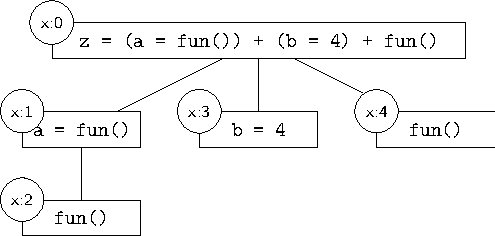
\includegraphics[width=0.5\textwidth]{scheme-generator/generated/label-hierarchy.pdf}
    \caption{\texttt{AbstractPoint} di un'istruzione alla linea $x$}
    \label{fig:realizzazione:label-hierarchy}
\end{figure}

\section{Control flow graph}

La classe \texttt{ControlFlowGraph} si occupa della costruzione del control flow graph a partire dall'albero sintattico astratto. Questa si appoggia sulla classe \texttt{MultiGraph} della libreria GraphStream anche per la visualizzazione. Sono possibili diversi \emph{layout} di visualizzazione a schermo, tra cui il layout gerarchico pensato appositamente per la presentazione del codice.

\section{Interprete}

L'interprete prende in input un control flow graph di Statement da eseguire. L'esecuzione si appoggia su una struttura ausiliaria detta \texttt{AbstractState} che sarà anche il risultato dell'operazione. 

L'interprete esegue anche in modo non deterministico le istruzioni del cfg aggiornando l'AbstractState. La classe \texttt{AbstractInterpreter} è incompleta, ed esegue le operazioni su oggetti astratti \texttt{AbstractValue}. Il programmatore dovrà definire il suo dominio di oggetti che ereditano da AbstractValue, le operazioni tra questi oggetti (i cui metodi sono elencati nella classe \texttt{AbstractDomainOperation}). Questi saranno poi passati al costruttore della classe AbstractInterpreter.

\subsection{\texttt{AbstractValue}}

L'interfaccia \texttt{AbstractValue} funge da segnaposto all'interno dei metodi che lavorano su oggetti del dominio astratto non ancora specificato. Un esempio di classi che la implementano sono \texttt{Top} e \texttt{Bottom}. 

Il programmatore specificherà poi il dominio sul quale vorrà lavorare. Noi utilizziamo per l'analisi il dominio SEA descritto in \cite{arceri}.

\subsection{\texttt{AbstractDomainOperation}}

L'interfaccia \texttt{AbstractDomainOperation} rappresenta una serie di operazioni che devono effettuare gli elementi del dominio. Una volta specificate le classi del dominio (es. SEA), dovrò creare una classe che implementa \texttt{AbstractDomainOperation} e che lavora in simbiosi con il dominio specificato.

\subsection{\texttt{AbstractState}}

La classe \texttt{AbstractState} rappresenta lo stato della computazione in ogni suo punto del codice. Il suo elemento principale è la classe \texttt{AbstractEnvironment}, cioè uno screenshot della memoria in un certo punto del codice (ad una certa linea, con una certa \emph{CallString} - vedi Sezione~\ref{sec:callstring}). L'\texttt{AbstractState} è quindi una mappa che associa ad una coppia $\struct{\ell, cs}$ un certo \texttt{AbstractEnvironment}.

\begin{figure}[htbp]
    \centering
    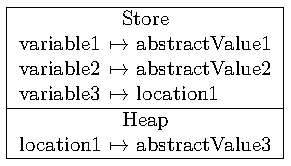
\includegraphics{scheme-generator/generated/environment.pdf}
    \caption{Struttura dell'\texttt{AbstractEnvironment}}
    \label{fig:realizzazione:abstractenvironment}
\end{figure}

L'\texttt{AbstractEnvironment} è formato da due strutture:
\begin{itemize}
    \item \texttt{AbstractStore}: mappa del tipo \texttt{Variable}$\mapsto$\texttt{AbstractValue} dove \texttt{Variable} è l'oggetto che denota una variabile; contiene le variabili globali e locali non allocate dinamicamente;
    \item \texttt{AbstractHeap}: mappa del tipo \texttt{AbstractLocation}$\mapsto$\texttt{AbstractValue} dove \texttt{AbstractLocation} è l'oggetto che denota un puntatore ad un oggetto.
\end{itemize}

\subsection{Dominio SEA}

Il dominio SEA utilizzato nella nostra analisi è formato da questi elementi:
\begin{itemize}
    \item \texttt{Interval}: intervallo di interi a 64-bit più due valori speciali $+\infty$ e $-\infty$;
    \item \texttt{Bool}: uno sei valori \texttt{TRUE}, \texttt{FALSE}, \texttt{UNKNOWN};
    \item \texttt{FiniteAutomata}: stringhe rappresentate come automi a stati finiti.
\end{itemize}
Oltre a questi elementi è presente anche la classe \texttt{AbstractObject} che fa parte come \texttt{AbstractValue} del dominio generico ed è comune a tutti i domini specificati dal programmatore. L'\texttt{AbstractObject} è una mappa di variabili in valori che implementa il concetto di proprietà dell'oggetto (Sezione~\ref{sec:js:createobj}). 

\subsection{Dichiarazioni ed assegnamenti}\label{sec:realizzazione:dichiarazioni}
\begin{javascriptcode}
var x = 2;
x = x + 2;
\end{javascriptcode}
La prima istruzione è una dichiarazione. Questa aggiunge la variabile \texttt{x} all'ambiente (Store) ed il suo valore astratto, considerando il dominio descritto precedentemente, è l'intervallo $[2,2]$ (cioè esattamente 2). L'ambiente modificato viene assegnato all'istruzione successiva \texttt{2:0}. Questa è un assegnamento, e modifica la variabile precedentemente dichiarata. L'ambiente che ne risulta viene assegnato ad \texttt{EOF}. 

\begin{figure}[htbp]
    \centering
    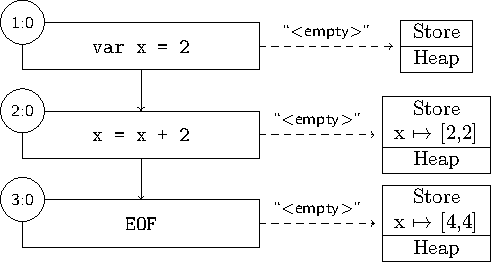
\includegraphics{scheme-generator/generated/example-declaration.pdf}
    \caption{Esempio della Sezione~\ref{sec:realizzazione:dichiarazioni}}
    \label{fig:realizzazione:dichiarazioni}
\end{figure}

Il risultato dell'esecuzione del codice sopra è visibile in Figura~\ref{fig:realizzazione:dichiarazioni}. Gli \texttt{AbstractEnvironment} delle istruzioni sono visibili a lato e connessi a queste tramite frecce tratteggiate. L'etichetta sulla freccia tratteggiata è chiamata \emph{call string} ed il suo significato può essere ignorato per il momento e verrà spiegato nella Sezione~\ref{sec:callstring}.

\subsection{Selezione}\label{sec:realizzazione:selezione}
\begin{javascriptcode}
var x = ..., y = 10; // x = 0 oppure x = 1
if(x == 0) {
    y = 5;
    x = y + 1;
} else {
    y = 33;
    x = y + 2;
}
\end{javascriptcode}
L'esecuzione del costrutto \texttt{if} parte con la valutazione della guardia. Se la guardia è sicuramente vera o sicuramente falsa, procediamo eseguendo la giusta diramazione. Quando non sappiamo con certezza questa cosa, dobbiamo eseguire separatamente.

\begin{figure}[htbp]
    \centering
    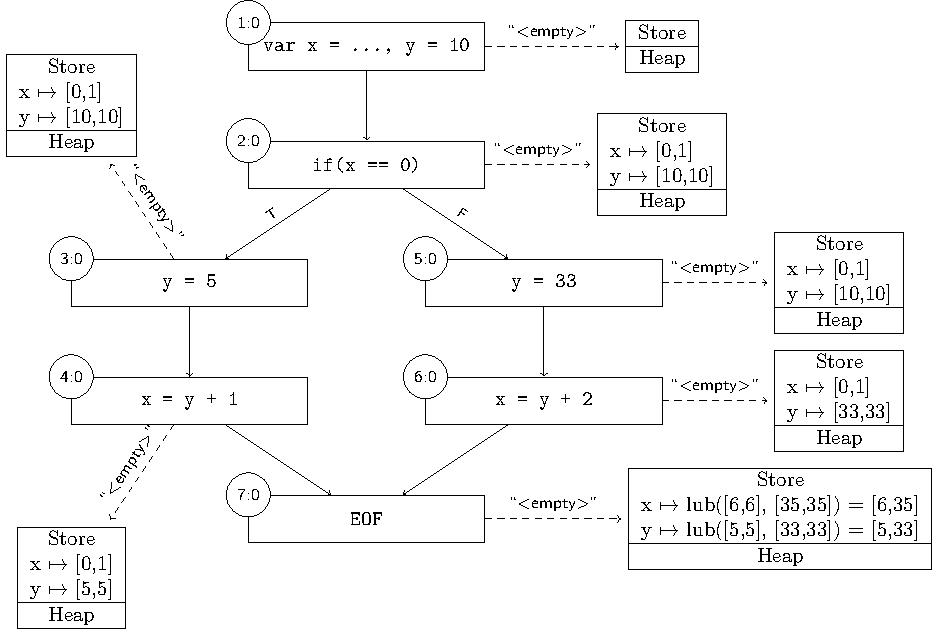
\includegraphics[width=\textwidth]{scheme-generator/generated/example-if.pdf}
    \caption{Esempio della Sezione~\ref{sec:realizzazione:selezione}}
    \label{fig:realizzazione:selezione}
\end{figure}

Nel codice sopra, quando valutiamo la guardia \texttt{x==0} questa potrebbe essere sia vera che falsa. Allora eseguiamo il branch ``vero" e ne mettiamo normalmente e ci salviamo a parte l'ambiente dopo aver eseguito l'ultima istruzione del branch ($e_1$). Eseguiamo poi allo stesso modo il branch ``falso" e, come per il precedente, mettiamo da parte l'ambiente dopo aver eseguito l'ultima istruzione del branch ($e_2$). L'ambiente della prima istruzione dopo il costrutto di selezione sarà $\join[e_1][e_2]$. 
Gli ambienti che risultano dall'esecuzione sono visibili in Figura~\ref{fig:realizzazione:selezione}.

\subsection{Iterazione}\label{sec:realizzazione:iterazione}
\begin{javascriptcode}
var x = 1;
while (x <= 3) {
    x = x + 1;
}
\end{javascriptcode}
Il costrutto \texttt{while} viene eseguito come segue parte con la valutazione della guardia. Se questa è falsa si continua con l'istruzione successiva. Altrimenti si esegue il corpo del while. Alla successiva iterazione, se la guardia potrebbe ancora essere vera, si esegue il widening del vecchio ambiente con il nuovo. Nel caso si raggiunga il fixpoint si continua con l'esecuzione, altrimenti si itera ancora. Gli ambienti che risultano dall'esecuzione sono visibili in Figura~\ref{fig:realizzazione:iterazione}.

\begin{figure}[htbp]
    \centerfloat
    \begin{subfigure}{.8\linewidth}
        \centering
        \fbox{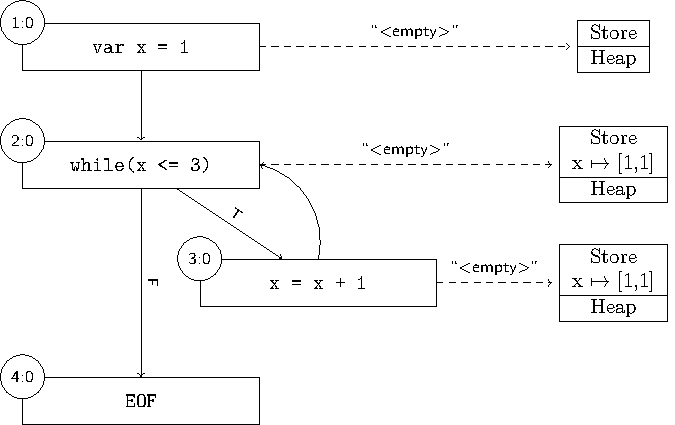
\includegraphics[width=0.8\textwidth]{scheme-generator/generated/example-while-1.pdf}}
        \caption{Prima iterazione}
        \label{fig:realizzazione:while-2}
    \end{subfigure}%
    \begin{subfigure}{.8\linewidth}
        \centering
        \fbox{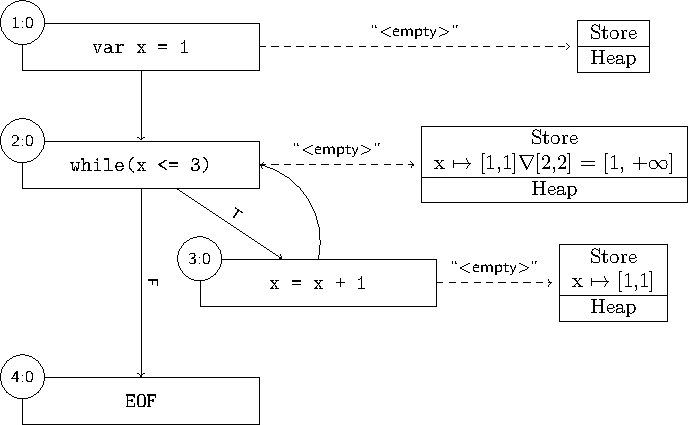
\includegraphics[width=0.8\textwidth]{scheme-generator/generated/example-while-2.pdf}}
        \caption{Seconda iterazione}
        \label{fig:realizzazione:while-2}
    \end{subfigure}\\[4ex]
    \begin{subfigure}{.8\linewidth}
        \centering
        \fbox{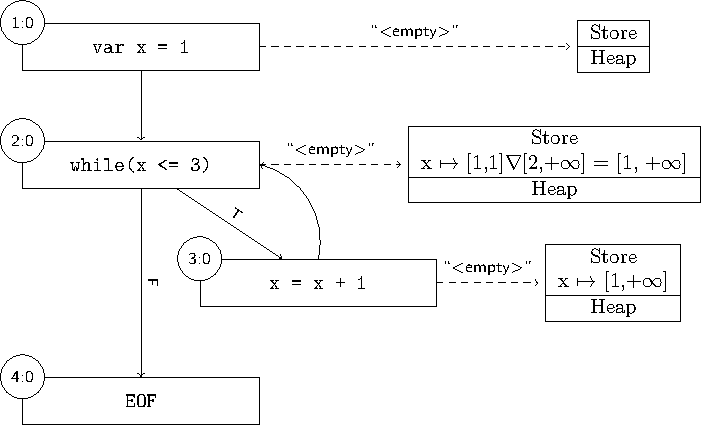
\includegraphics[width=0.8\textwidth]{scheme-generator/generated/example-while-3.pdf}}
        \caption{Terza iterazione}
        \label{fig:realizzazione:while-2}
    \end{subfigure}%
    \begin{subfigure}{.8\linewidth}
        \centering
        \fbox{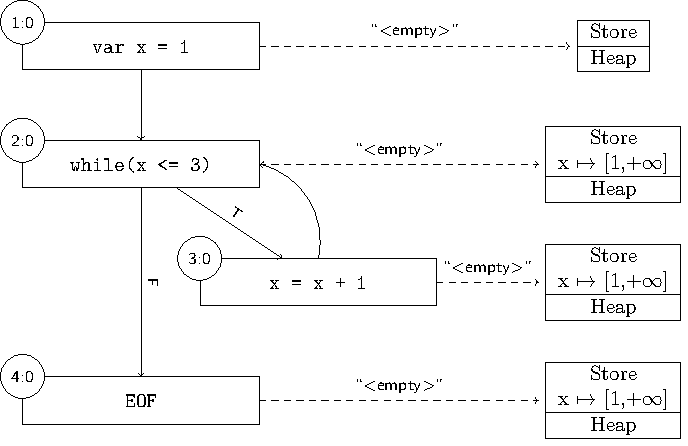
\includegraphics[width=0.8\textwidth]{scheme-generator/generated/example-while-4.pdf}}
        \caption{Completo}
        \label{fig:realizzazione:while-2}
    \end{subfigure}%
    \caption{Esempio della Sezione~\ref{sec:realizzazione:iterazione}}
    \label{fig:realizzazione:iterazione}
\end{figure}

\subsection{Chiamate a funzione}\label{sec:callstring}

Ogni funzione è definita da un control flow graph con una prima istruzione segnaposto detta \emph{entry point} ed un'ultima istruzione segnaposto detta \emph{exit point}.

Quando incontro la definizione di funzione, questa viene aggiunta all'ambiente in tre passi:
\begin{enumerate}
    \item aggiungo allo store un binding di tipo \emph{nome funzione} $\mapsto$ \emph{insieme di locazioni}, dove ogni locazione è un riferimento ad un oggetto nell'heap; se è già presente un binding con chiave \emph{nome funzione} allora passo al punto successivo;
    \item genero una locazione per un oggetto \texttt{AbstractFunction} che conterrà la definizione della funzione incontrata; aggiungo all'heap un binding di tipo \emph{locazione} $\mapsto$ \emph{definizione di funzione};
    \item aggiungo allo store, all'entry di chiave \emph{nome funzione}, la locazione generata nel punto precedente al corrispondente insieme di locazioni.
\end{enumerate}

Quando incontro la chiamata a funzione connetto \emph{dinamicamente} la chiamata agli entry point ed exit point della funzione. Prima della chiamata valuto gli argomenti della funzione. Alla funzione passo poi l'ambiente nel punto precedente della chiamata più gli argomenti valutati all'\emph{entry point}. Al termine della chiamata ritorna un valore. 

\subsubsection{Chiamata a funzioni na\"ive} 

Eseguiamo le funzioni come se fossero un normale pezzo di codice. Con questo metodo ad ogni chiamata di funzione possiamo perdere precisione. Viene introdotto il metodo delle CallString.

\subsubsection{Chiamata a funzione con call string}\label{sec:callstring:internal}
\begin{javascriptcode}
function add(n,m) {
    return n + m;
}
var x = add(1000, 1);
var y = add(-500, 1);
\end{javascriptcode}
Il metodo delle call string permette di aumentare la precisione delle chiamate a funzione. Occorre differenziare gli ambienti delle istruzioni della funzione a seconda di chi l'ha chiamata.

Le chiamate vengono identificate grazie all'identificatore che hanno le istruzioni, visibile all'interno degli schemi nel cerchio alla loro destra. L'identificatore dell'istruzione è ovviamente univoco.

\begin{figure}[htbp]
    \centering
    \begin{subfigure}{\linewidth}
        \centering
        \fbox{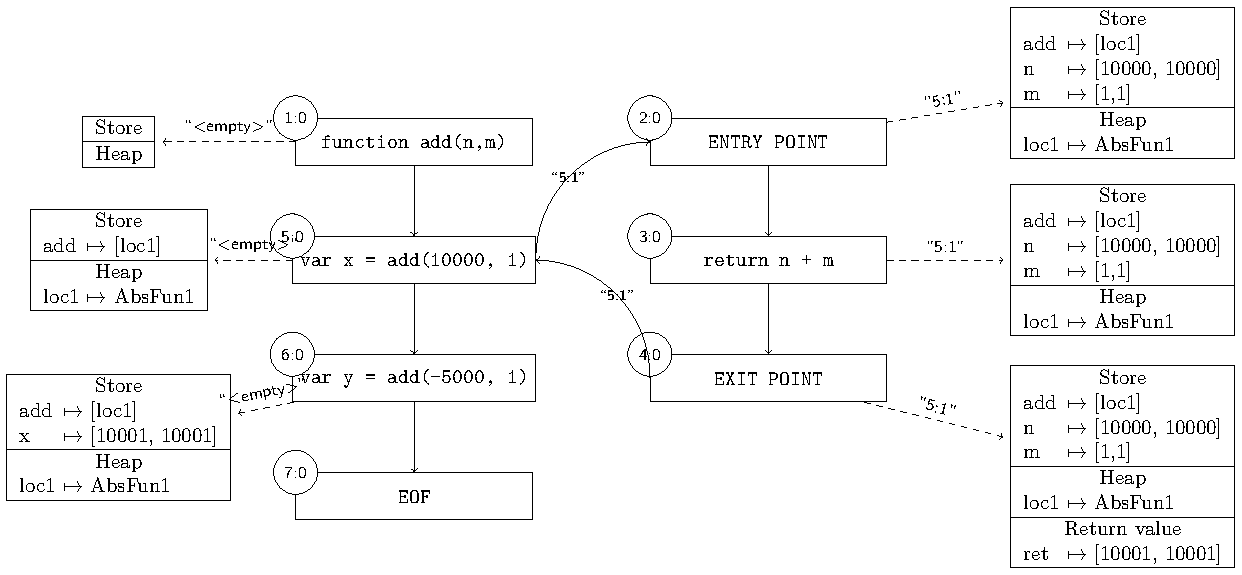
\includegraphics[width=\textwidth]{scheme-generator/generated/example-fun-cs-1.pdf}}
        \caption{Dopo la prima chiamata}
    \end{subfigure}\\[4em]
    \begin{subfigure}{\linewidth}
        \centering
        \fbox{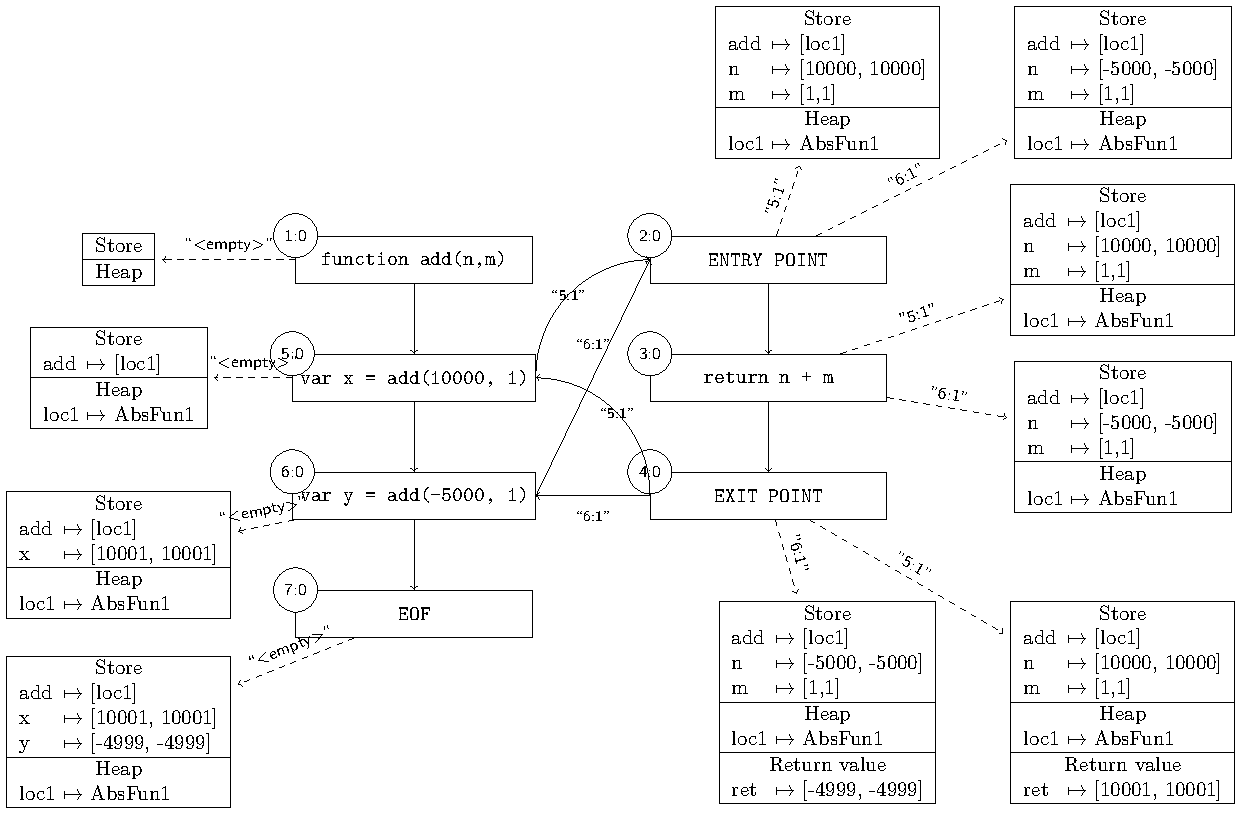
\includegraphics[width=\textwidth]{scheme-generator/generated/example-fun-cs-2.pdf}}
        \caption{Dopo la seconda chiamata}
    \end{subfigure}
    \caption{Esempio della Sezione~\ref{sec:callstring:internal}}
    \label{fig:realizzazione:callstring:internal}
\end{figure}

\subsection{Chiamate a funzione ricorsive}\label{sec:realizzazione:recursive}
\begin{javascriptcode}
function fact(n) {
    if(n <= 1) {
        return 1;
    } else {
        return n * fact(n-1);
    }
}
var result = fact(5);
\end{javascriptcode}
Una call string è quindi formata da una sequenza di chiamata a funzione. Se consideriamo le call string come illimitate, cioè che possiamo tenere in memoria un numero illimitato di sequenze di chiamata a funzione, la nostra analisi potrebbe divergere. Fissiamo quindi una lunghezza massima di call string pari a 2. 

Quando una callstring \textsf{``c1:c2:...:cn"} ha raggiunto la sua lunghezza massima, la sua concatenazione con una chiamata \textsf{cm} risulta in \textsf{``c2:...:cn:cm"}, cioè viene eliminata la sua chiamata più vecchia. Ricorda che ad ogni statement, ad ogni callstring, è associato un ambiente.

Prendiamo per esempio il codice seguente che implementa la funzione ricorsiva fattoriale. L'esecuzione della prima e seconda chiamata è simile all'esempio non ricorsivo. Arrivato alla terza chiamata, la call string \textsf{``6:1,5:1,5:1"} viene approssimata ed otteniamo \textsf{``5:1,5:1"}. Alla quarta chiamata abbiamo la call string \textsf{``5:1,5:1,5:1"} approssimata a \textsf{``5:1,5:1"}. Ci accorgiamo che è già presente un ambiente associato all'istruzione con quella call string ed applichiamo il widening tra i due ambienti. Il parametro $n$ prende il valore di $n = [3,3] \nabla [2,2] = [-\infty,3]$. Questa parte di esecuzione è visibile in Figura~\ref{fig:realizzazione:fun-hierarchy-1}.

\begin{figure}[htbp]
    \centering
    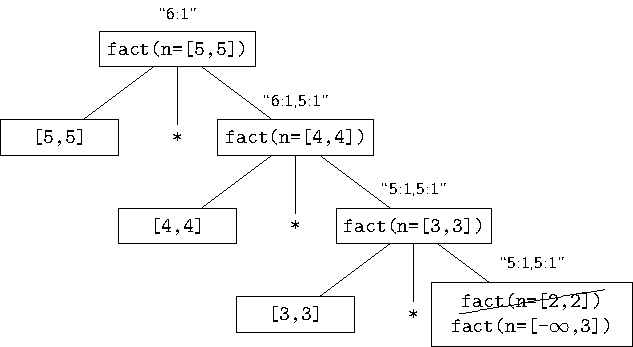
\includegraphics[width=0.8\textwidth]{scheme-generator/generated/example-fun-rec-hierarchy-1.pdf}
    \caption{Prima parte}
    \label{fig:realizzazione:fun-hierarchy-1}
\end{figure}

A questo punto dobbiamo controllare se abbiamo \emph{raggiunto il fixpoint}, cioè se l'ambiente precedente al widening (con $n=[3,3]$) e quello del widening (con $n = [-\infty, 3]$) sono uguali. Non lo sono, quindi continuo l'esecuzione.

Questa chiamata porta ad avere due diramazioni: una ritorna il valore $[1,1]$ ed un altra continua ricorsivamente. Il valore di ritorno viene \emph{salvato} all'interno dell'ambiente dell'istruzione dell'ultima chiamata a funzione con la call string corrente. Ora, quando incontreremo una chiamata a funzione già calcolata (fixpoint) ritorneremo questo valore al posto che eseguire ancora la funzione. Questa parte di esecuzione è visibile in Figura~\ref{fig:realizzazione:fun-hierarchy-2}.

\begin{figure}[htbp]
    \centering
    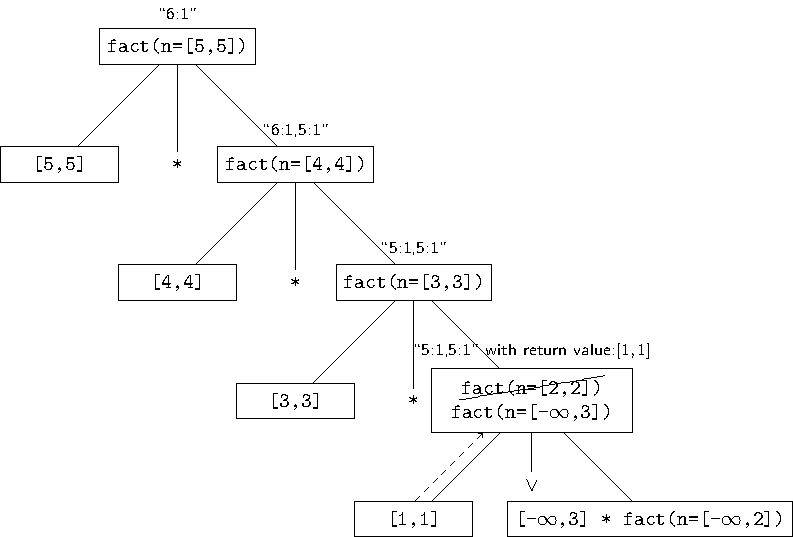
\includegraphics[width=0.8\textwidth]{scheme-generator/generated/example-fun-rec-hierarchy-2.pdf}
    \caption{Seconda parte}
    \label{fig:realizzazione:fun-hierarchy-2}
\end{figure}

L'altra diramazione porta alla chiamata ricorsiva di \texttt{fact}. La call string dopo l'approssimazione è sempre \textsf{``5:1,5:1"}. Applichiamo il widening dei due ambienti, $n$ prende il valore $[-\infty,3]\nabla[-\infty,2]=[-\infty,3]$. Abbiamo raggiunto il fixpoint quindi \emph{non continuiamo l'esecuzione} ma la blocchiamo. Ritorniamo il valore di ritorno associato all'ambiente, che in questo caso è $[1,1]$.  Questa parte di esecuzione è visibile in Figura~\ref{fig:realizzazione:fun-hierarchy-3}.

\begin{figure}[htbp]
    \centering
    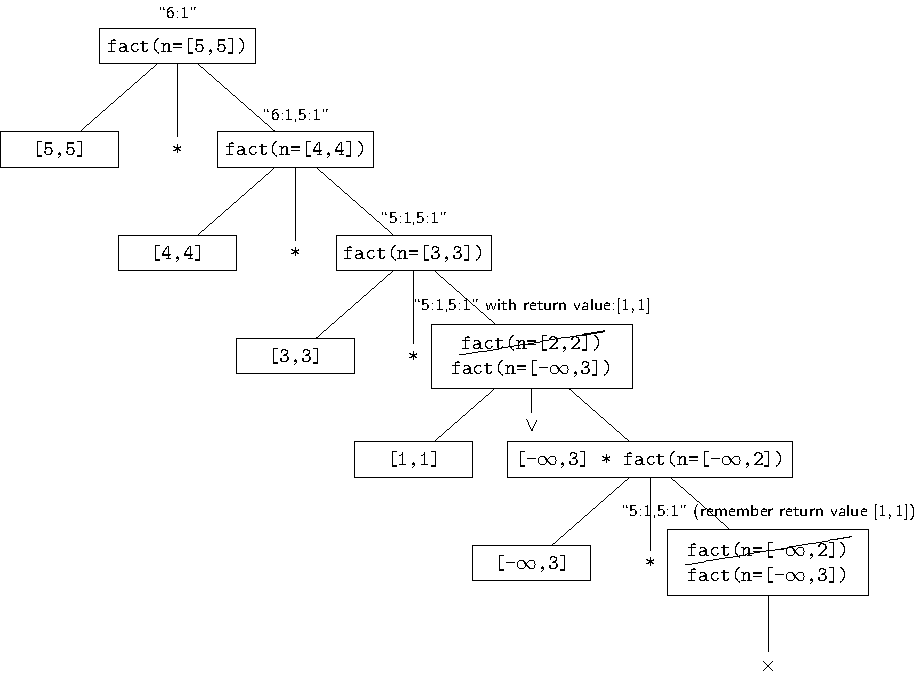
\includegraphics[width=0.8\textwidth]{scheme-generator/generated/example-fun-rec-hierarchy-3.pdf}
    \caption{Terza parte}
    \label{fig:realizzazione:fun-hierarchy-3}
\end{figure}

Ora che ho finito l'esecuzione risalgo l'albero di chiamate ritornando i valori richiesti ai chiamanti. Il risultato finale di \texttt{fact(5)} è un numero compreso nell'intervallo $[-\infty,180]$, coerente col vero valore $5!=120$. L'esecuzione di quest'ultimo step è visibile in Figura~\ref{fig:realizzazione:fun-hierarchy-4}.

\begin{figure}[htbp]
    \centering
    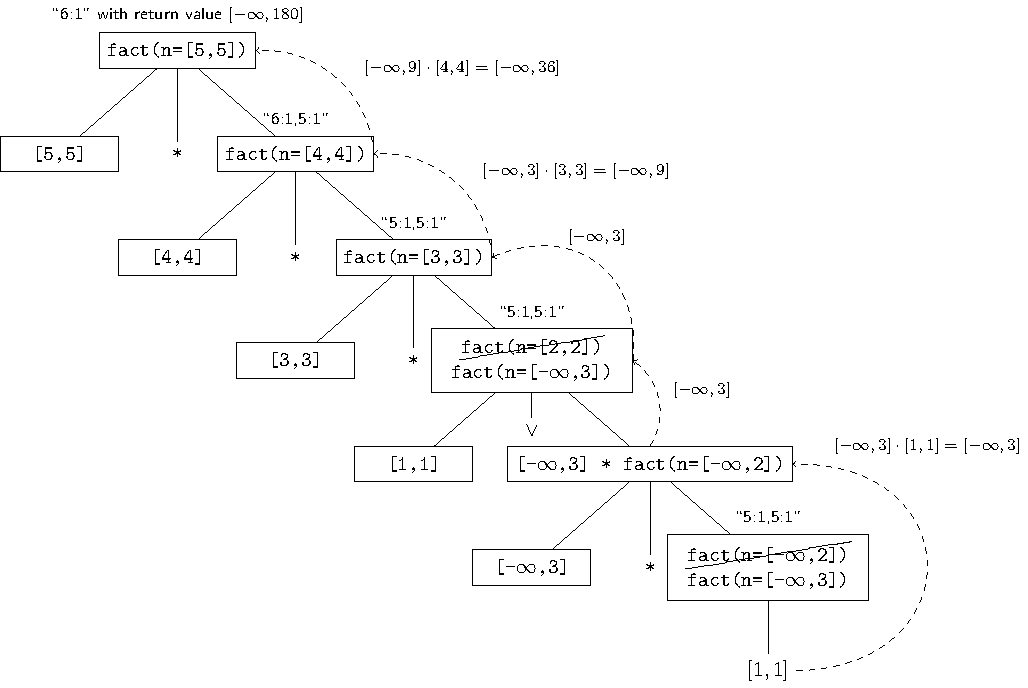
\includegraphics[width=0.8\textwidth]{scheme-generator/generated/example-fun-rec-hierarchy-4.pdf}
    \caption{Completo}
    \label{fig:realizzazione:fun-hierarchy-4}
\end{figure}


\begin{appendices}
\newcommand{\uco}{\fun{uco}}
\newcommand{\lfp}{\fun{lfp}}

\chapter{Teoria dei reticoli}\label{chap:teoriareticoli}

\section{Poset}

\begin{definition}[Poset]
Un \emph{insieme parzialmente ordinato} o \emph{poset} è una struttura $\struct{P, \sqsubseteq}$ tale che $P$ è un insieme e $\sqsubseteq$ è una relazione binaria su $P$ che gode di proprietà \emph{riflessiva}, \emph{antisimmetrica} e \emph{transitiva}. 
\end{definition}

In una relazione d'ordine parziale $\sqsubseteq$ non è detto che tra due elementi $x,y \in P$ questi siano confrontabili, cioè che valga $x \sqsubseteq y \lor y \sqsubseteq x$. In questo caso si scrive $x || y$. Se tutti gli elementi dell'insieme sono a due a due confrontabili, la relazione d'ordine si dice \emph{totale} e viene indicata col simbolo $\le$. 

Esempi di poset le strutture $\struct{\mathbb{Z}, \le}$ (che è anche un insieme totalmente ordinato), la struttura $\struct{\wp(S), \subseteq}$ formata dall'insieme delle parti di un insieme $S$ e la relazione di inclusione insiemistica (Figura~\ref{fig:poset-parti}), ma anche la struttura $\struct{\{1,2,3,4,6,12\}, \mathbf{divide}}$.

\begin{figure}[htbp]
    \centering
    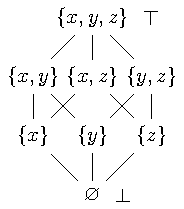
\includegraphics{appendici/immagini/poset-parti.pdf}
    \caption{Poset $\struct{\wp(S), \subseteq}$ con $S = \{x,y,z\}$}
    \label{fig:poset-parti}
\end{figure}

\begin{definition}[Elementi top e bottom]
All'interno di un poset $\struct{P, \sqsubseteq}$ si può individuare, se esiste, l'elemento top $\top \in P$ tale che $\forall x \in P . x \le \top$. Se l'elemento $\top$ esiste, è unico. L'elemento bottom $\bot$ è definito in modo duale.
\end{definition}

All'interno del poset $\struct{\wp(S), \subseteq}$ l'elemento top è $\top = S$ e il bottom è $\bot = \varnothing$. All'interno del poset $\struct{\mathbb{Z}, \le}$ non esiste l'elemento top ma esiste l'elemento bottom $\bot = 0$. Se ad $\mathbb{Z}$ aggiungiamo un ulteriore elemento $\infty$ tale che $\forall n \in \mathbb{Z} . n < \infty$ allora questo elemento funge da top per la nuova struttura $\struct{\mathbb{Z} \cup \{ \infty \}, \le}$ creata.

\begin{definition}[Least upper bound]
L'operazione di \emph{least upper bound} (o \emph{lub}, \emph{join}, \emph{estremo superiore}) tra due elementi $x,y \in P$ di un poset $\struct{P, \sqsubseteq}$ se esiste è l'elemento $\join[x][y] = z \in P$ tale che:
\begin{itemize}
    \item $\join[x][y]$ è maggiorante di $x$ e $y$ ($x,y \sqsubseteq \join[x][y]$);
    \item $\join[x][y]$ è il più piccolo maggiorante di $x$ e $y$ ($\forall m \in P . (x,y \sqsubseteq m \to \join[x][y] \sqsubseteq m)$);
    \item $\join[x][y]$ è unico.
\end{itemize}
\end{definition}

\begin{definition}[Greatest lower bound]
L'operazione di \emph{greatest lower bound} (o \emph{glb}, \emph{meet}, \emph{estremo inferiore}) è definito in modo duale al lub e di indica con $\meet[x][y]$ per $x,y \in P$.
\end{definition}

Il join (e il meet) di due elementi del poset può non essere definito per due motivi: \emph{l'elemento manca} (in $\struct{\{1,2,3,4,6,12,13\}, \mathbf{divide}}$ l'elemento $\join[12][13]$ non è definito poichè non c'è elemento maggiorante di entrambi) oppure \emph{non è rispettata la condizione di unicità} (se ci sono più maggioranti non confrontabili tra loro).

\begin{definition}[Catena]
Un sottoinsieme $C \subseteq P$ del poset $\struct{P, \sqsubseteq}$ è detto \emph{catena} se gli elementi di $C$ sono a due a due confrontabili tra loro. Il duale della catena è l'anticatena (elementi non confrontabili tra loro).  
\end{definition}

\begin{definition}[Condizione ACC]
Una catena $C$ soddisfa la \emph{ascending chain condition} se $C$ è un insieme finito oppure se da un certo $n$ in poi si ha $\forall m > n . c_n = c_m$.
\end{definition}

\begin{definition}[Poset completo]
Un poset $\struct{P, \sqsubseteq}$ si dice completo (abbreviato \emph{c.p.o.}) se per ogni sua catena $C$ anche infinita esiste l'estremo superiore $\join[C] \in P$.
\end{definition}

\subsection{Reticoli}\label{sec:reticoli}

\begin{definition}[Reticolo]
Un reticolo è una struttura $\struct{P, \sqsubseteq, \join, \meet}$ nella quale $\struct{P, \sqsubseteq}$ è un poset, l'operazione binaria $\join$ effettua il lub, l'operazione $\meet$ effettua il glb ed 
\[ \forall x,y \in P \text{ sono definiti } \join[x][y], \meet[x][y] \in P \]
\end{definition}

\begin{definition}[Sottoreticolo]
Un sottoinsieme $Q \subseteq P$ del reticolo $\struct{P, \sqsubseteq, \join, \meet}$ è detto \emph{sottoreticolo} se $Q$ è chiuso per lub e glb ($\forall x,y \in Q . \join[x][y], \meet[x][y] \in Q$). 
\end{definition}

\begin{definition}[Reticolo completo]
Un reticolo che è anche c.p.o. viene detto reticolo completo.
\end{definition}

\subsection{Ordinamento pointwise di funzioni}

Date due funzioni $f_1, f_2 : C \to C$, il loro ordinamento parziale $\le$ è detto \emph{pointwise} se
\[ f_1 \le f_2 \iff \forall x \in C . f_1(x) \le f_2(x) \]

\subsection{Connessione di Galois}\label{sec:galois}

La definizione di connessione di Galois è presente alla Sezione~\ref{sec:galois-c}.

\begin{theorem}[Connessione di Galois come adjunctor]
La struttura è detta anche \emph{adjunctor} ($\alpha$ left adjoint, $\gamma$ right adjoint) poichè vale che
$$\forall c \in C, a \in A \; : \; \alpha(c) \preceq a \Leftrightarrow c \le \gamma(a)$$
\end{theorem}

\begin{theorem}[Connessione di Galois come funzioni additive e co-additive]
In una connessione di Galois la funzione $\alpha$ è additiva, cioè preserva l'operazione di join: 
$$\alpha\left(\join[X]\right) = \join[\alpha(X)] \text{ per ogni } X \subseteq C$$
e la funzione $\gamma$ è co-additiva, cioè preserva l'operazione di meet.
\end{theorem}

\begin{definition}[Inserzione di Galois]
Una connessione di Galois si dice \emph{inserzione di Galois} e si scrive $C \galoiS{\alpha}{\gamma} A$ se $\alpha \circ \gamma = \fun{id}$. Sono equivalenti le seguenti espressioni:
\begin{itemize}
    \item $C \galoiS{\alpha}{\gamma} A$;
    \item $\alpha$ è suriettiva;
    \item $\gamma$ è iniettiva.
\end{itemize}
\end{definition}

Le inserzioni di Galois sono molto simili alle connessioni. La differenza tra i due è che nelle connessioni è possibile che più elementi del dominio astratto corrispondano allo stesso elemento del dominio concreto. Togliendo questi elementi ``superflui" si ottiene una inserzione. Questo procedimento, detto \emph{reduction} è sempre possibile e consiste nell'identificare in una classe di equivalenza gli elementi del dominio astratto con la stessa concretizzazione.

\section{Closure operators}

Un'interpretazione astratta può essere definita equivalentemente come una inserzione di Galois oppure come un'operatore di chiusura. La teoria di questa sezione è presa da \cite{ranzato}, che espone questi concetti in modo più approfondito. 

\begin{definition}[Upper closure operator]
Una funzione $\rho: L \to L$ è detta \emph{upper closure operator} se
\begin{enumerate}
    \item monotona: $x \le y \to \rho(x) \le \rho(y)$;
    \item estensiva: $x \le \rho(x)$;
    \item idempotente: $\rho(\rho(x)) = \rho(x)$.
\end{enumerate}
\end{definition}

Dato un reticolo completo $C$, un'operatore di chiusura $\rho$ è determinato univocamente dalla sua immagine $\rho(C) = \mathrm{codomain}(\rho)$. L'immagine di un $\rho$ coincide con l'insieme dei suoi \emph{fixpoint}:
\[ \rho(y) = \meet[\{x \mid x \in \mathrm{codomain}(\rho) \land y \le x \}] \]

\begin{definition}[Famiglia di Moore]
Un sottoinsieme $X \subseteq L$ di un reticolo completo $L$ è detto \emph{famiglia di Moore} se $X$ è chiuso rispetto all'operazione di \emph{meet}, cioè
$$X = \mathcal{M}(X); \qquad \mathcal{M}(X) = \Big\{ \meet[S] \; \big| \; S \subseteq X \Big\}$$
\end{definition}

Viceversa, un'operatore $\rho$ sul dominio $J$ è un $\uco$ se e solo se il suo codominio $\rho(J) = K$ è una famiglia di Moore ed in quel caso $\rho(y) = \meet[\{x \mid x \in K \land y \le x \}]$. 

\subsection{Reticolo delle interpretazioni astratte}

Se $C$ è un reticolo completo, allora $\uco(C)$ forma un reticolo completo rispetto all'ordinamento pointwise con elemento $\top = \lambda x . \top$ e $\bot = \lambda x . x$. 

Dato $\rho \in \uco(C)$ ed un dominio astratto $A$, se $\rho(C)$ è isomorfico ad $A$ abbiamo $\iota: \rho(C) \to A$ ed $\iota^{-1} : A \to \rho(C)$. Allora la struttura
\[ \struct{\iota \circ \rho, C, A, \iota^{-1}} \]
è un'inserzione di Galois. Allo stesso tempo se $\struct{\gamma, C, A, \alpha}$ è un'inserzione di Galois allora $\rho_{A} = \gamma \circ \alpha$ è un $\uco(C)$.  

Definiamo l'insieme $\mathrm{Abs}(C)$ come l'insieme dei domini astratti di $C$. L'insieme forma un reticolo completo rispetto all'operazione di ordinamento
\[ A_1 \sqsubseteq A_2 
\iff \rho_{A_1} \subseteq \rho_{A_2} 
\iff \left( 
    \forall x . \rho_{A_1}(x) \le \rho_{A_2}(x)
\right) \]
e nel caso si dice che $A_1$ è più preciso (o più concreto) di $A_2$. La struttura $\struct{\mathrm{Abs}(C), \sqsubseteq}$ forma un reticolo completo detto \emph{reticolo delle interpretazioni astratte} ed è isomorfico al reticolo $\struct{\uco(C), \sqsubseteq}$. 

\section{Fixpoint}\label{sec:fixpoint}

\begin{definition}[Fixpoint]
Data $f:X \to X$, il punto $x \in X$ si definisce fixpoint se $f(x) = x$.
\end{definition}

\begin{definition}[Least fixed point]
Data $f:X \to X$, il punto $\lfp(f) = x \in X$ si definisce \emph{least fixed point} se per ogni $y$ fixpoint si ha $x \le y \to x = y$.
\end{definition}

\begin{theorem}[Teorema di Knaster-Tarski]
Data una funzione $f:L \to L$ monotona su un reticolo completo $\struct{L, \le}$ esiste un unico $\lfp(f)$.
\end{theorem}

E' possibile calcolare $\lfp(f)$ tramite il metodo iterativo:
$$\bot \le f(\bot) \le f^2(\bot) \le ... \le f^n(\bot) = \lfp(f) = f^{n+1}(\bot) = f^{n+2}(\bot) = ...$$

\section{Widening}

I domini concreti $C$ possono avere infiniti valori. I domini astratti che abbiamo visto possono avere valori finiti (dominio dei segni) o infiniti (dominio degli intervalli). A volte non è possibile garantire la convergenza dei calcoli su domini infiniti (non rispettando la condizione di ACC). Si definisce allora una funzione detta widening che garantisce la terminazione a costo di perdere ulteriore precisione.

\begin{definition}[Widening binario]
L'operatore di widening $\wide: P \times P \to P$ su un poset $\struct{P, \le}$ soddisfa le seguenti condizioni:
\begin{itemize}
    \item $\forall x,y \in P \, . \, x \le (\wide[x][y]) \land y \le (\wide[x][y])$;
    \item Per ogni catena $x_0 \le x_1 \le ...$ si definisce la catena \emph{non strettamente crescente} $y_0 = x_0, ..., y^{n+1} = \wide[x][y^n]$.
\end{itemize}
\end{definition}

L'operatore di widening non è commutativo ne associativo. L'iterazione col widening si svolge come segue:
$$x^0 = \bot \qquad x^{n+1} = \begin{cases} 
    x^n,                & f(x^n) \le x^n \\ 
    \wide[x^n][f(x^n)], & f(x^n) \not\le x^n \\
\end{cases}$$

\end{appendices}

\printbibliography

\end{document}
